\newpage
\subsection{Arquitectura de la aplicación móvil}

La aplicación móvil constituirá la principal herramienta de trabajo en campo para la recolección de datos y el análisis de los árboles. Estará diseñada de forma nativa para el sistema operativo Android, priorizando la eficiencia en el consumo de recursos (batería y memoria) y la capacidad de operar de manera autónoma sin depender de conectividad a la red.

\subsubsection{Componentes de la aplicación}

El desarrollo de la aplicación se realizará utilizando \textbf{Kotlin} como lenguaje de programación principal, alineándose con los estándares modernos y las recomendaciones oficiales de Google para el desarrollo nativo en Android. 

Para el diseño y la construcción de la interfaz gráfica, se prescindirá del sistema tradicional de vistas basadas en XML en favor de \textbf{Jetpack Compose}. Este \textit{toolkit} de UI declarativa permitirá construir interfaces reactivas, escalables y modulares, reduciendo significativamente la cantidad de código y facilitando la gestión del estado de la aplicación en pantallas complejas, como la vista de captura fotográfica y el despliegue de resultados.

La arquitectura interna de la aplicación seguirá el patrón de diseño \textit{Model-View-ViewModel} (MVVM), recomendado para el ecosistema Android. Esto garantizará una estricta separación de responsabilidades entre la lógica de presentación (gestionada por Compose), la lógica de preparación de datos (\textit{ViewModels}) y la lógica de acceso a datos (\textit{Repositories}).

\subsubsection{Inferencia local y procesamiento de imágenes}

La característica central del cliente móvil será su capacidad de analizar fotografías para detectar la presencia de insectos descortezadores de manera estrictamente local (\textit{on-device}). Este enfoque eliminará la latencia de red y permitirá que el sistema funcione en zonas boscosas sin cobertura.

Es imperativo señalar que el análisis de cada fotografía se ejecutará \textbf{una única vez} en el dispositivo. El sistema no realizará reevaluaciones posteriores sobre la misma imagen una vez que se haya emitido el diagnóstico inicial, garantizando así un uso eficiente de la batería y del poder de cómputo del teléfono. El flujo de este procesamiento único constará de dos etapas fundamentales:

\begin{enumerate}
    \item \textbf{Preprocesamiento con OpenCV:} Al momento de la captura, la imagen pasará por una tubería de preprocesamiento utilizando la librería OpenCV para Android. Esta etapa incluirá técnicas de análisis cromático y filtrado de ruido para resaltar las áreas de interés (e.g., manchas de resina o aserrín en la corteza), además de redimensionar y normalizar los tensores para que coincidan con la entrada de la red neuronal.
    \item \textbf{Inferencia con TensorFlow Lite:} La imagen procesada será evaluada de inmediato por el modelo de Deep Learning (basado en arquitecturas eficientes como EfficientNet-B3 o YOLO), el cual estará integrado en la aplicación en formato \texttt{.tflite}. La API de \textbf{TensorFlow Lite} aprovechará la aceleración de \textit{hardware} del dispositivo para emitir el diagnóstico en tiempo real. Este resultado quedará asociado de forma permanente al registro de la captura.
\end{enumerate}


\subsubsection{Estrategia \textit{Offline-First} y sincronización}

Para garantizar la integridad y la persistencia de los diagnósticos generados en áreas sin internet, la aplicación implementará una estricta estrategia \textit{Offline-First}. Bajo este paradigma, el dispositivo móvil actuará como la fuente primaria de verdad a corto plazo.

La persistencia local de los datos estructurados (información del árbol, coordenadas geográficas, fecha y el diagnóstico único emitido por TFLite) se gestionará utilizando \textbf{SQLite} a través de la librería \textbf{Room}. Room proporcionará una capa de abstracción robusta, verificando las consultas SQL en tiempo de compilación y exponiendo los datos mediante flujos asíncronos (\textit{Coroutines} y \textit{Flows} de Kotlin). Las imágenes asociadas a cada reporte se almacenarán de forma segura en el almacenamiento interno del dispositivo.

Cuando el sistema operativo notifique a la aplicación sobre la disponibilidad de una conexión a internet estable, se detonará un proceso en segundo plano (\textit{background worker}) para sincronizar los registros locales pendientes con la nube. 

Para estas comunicaciones de red, se utilizará la combinación de \textbf{Retrofit} y \textbf{OkHttp}. Retrofit facilitará la construcción de las peticiones REST hacia Amazon API Gateway. Por su parte, OkHttp se empleará para interceptar estas peticiones e inyectar automáticamente el \textbf{token JWT propio} en las cabeceras HTTP de autorización. Una vez que el \textit{backend} en AWS confirme la recepción e inserción exitosax de los datos (HTTP 200), la aplicación actualizará el estado de los registros en SQLite como "sincronizados", completando así el ciclo de vida de la información capturada en campo.

\begin{figure}[H]
    \centering
    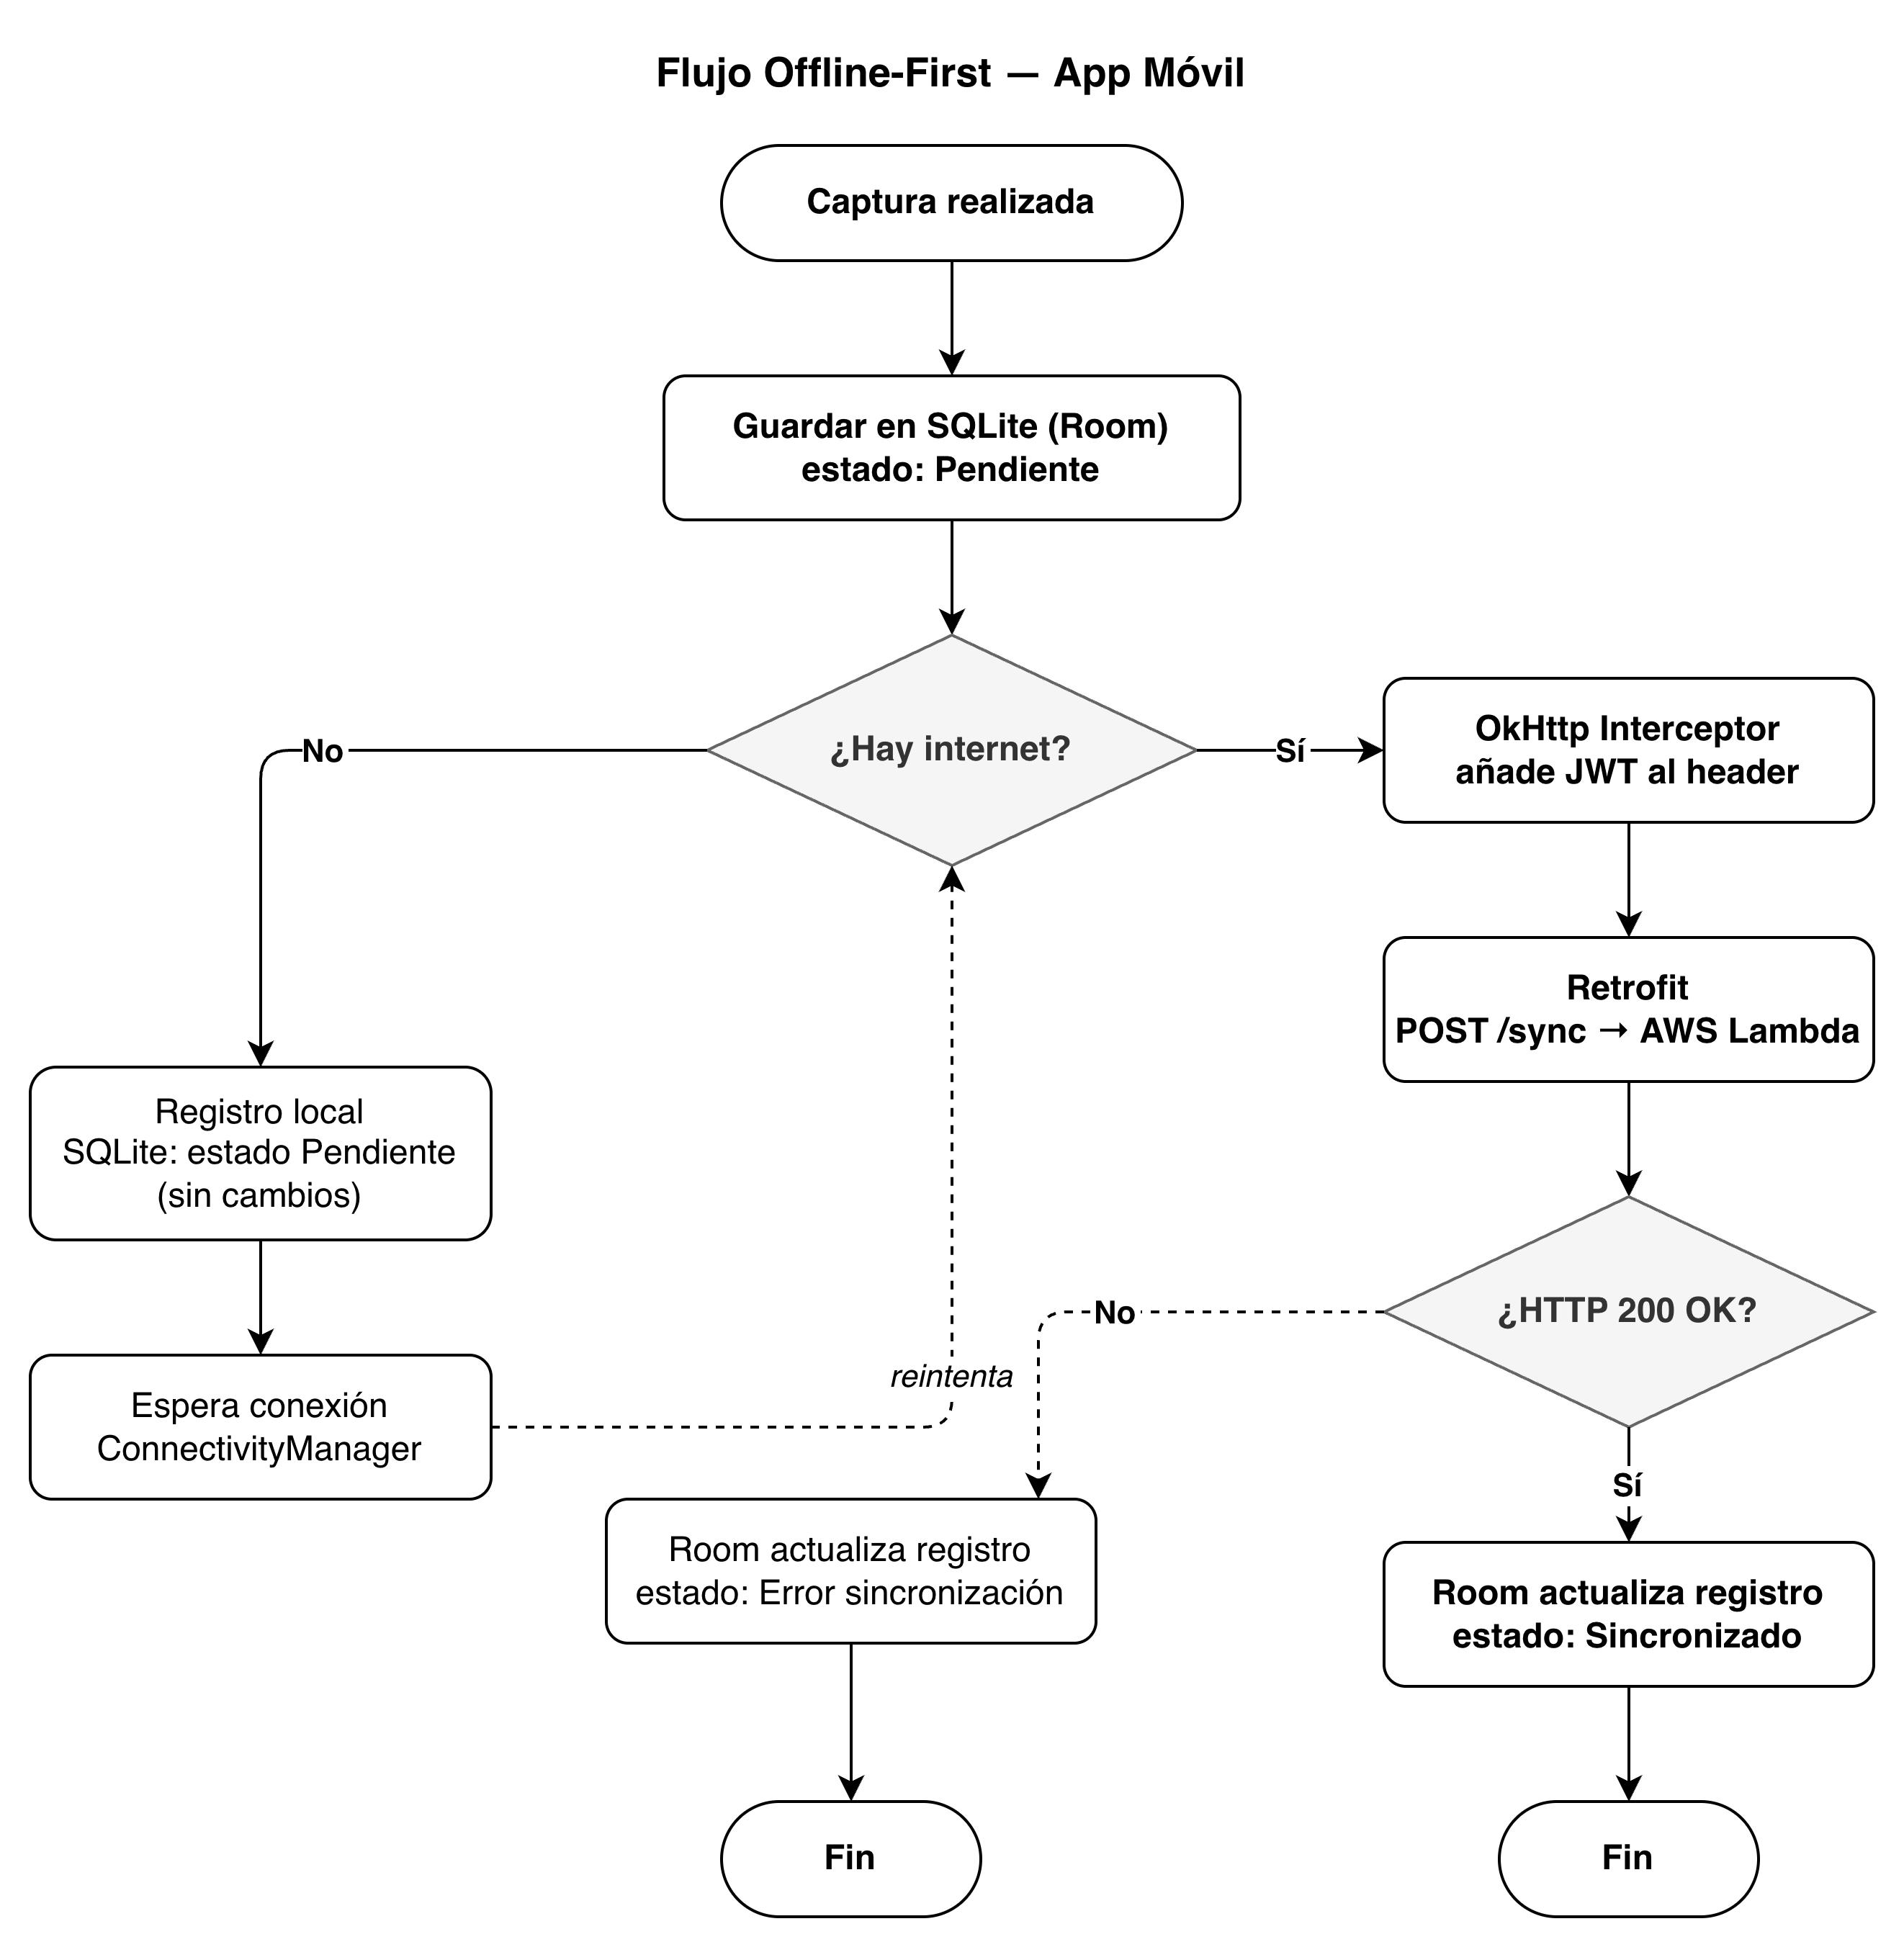
\includegraphics[width=0.8\textwidth]{images/C8/offline.jpeg}
    \caption{Flujo de decisión y sincronización de datos de la estrategia \textit{Offline-First}.}
    \label{fig:flujo-offline-first}
\end{figure}